
%% F?r die endg?ltige Version von ``draft'' auf ``final'' umstellen
\documentclass[12pt,headsepline,twoside,draft]{scrreprt}
\usepackage[utf8]{inputenc}
\usepackage[T1]{fontenc}



\usepackage{templates/kitreport}
\usepackage{templates/listings}
\usepackage{templates/tikzkit}
\usepackage{templates/tikzuml}
\usepackage{import}
\usepackage{xspace}
\usepackage{pdfsync}
\usepackage{changes}
\usepackage{wrapfig}
\usepackage{subfigure}
\usepackage{rotating}
\usepackage{pdflscape}
\usepackage{enumitem}
\usepackage{longtable}
\usepackage{booktabs}
\usepackage{hyperref}
\usepackage[section]{placeins}
\usepackage{todonotes}
\newcommand{\todosk}[1]{\todo[inline, color=teal!31]{TODO: #1}}
\newcommand{\CoCoME}{\mbox{CoCoME}\xspace}
\newcommand{\CoCoMEP}{\mbox{CoCoMEP}\xspace}
\newcommand{\textcode}[1]{\textsf{\footnotesize #1}}
\usepackage{makecell}


%Draft Watermark
\usepackage{draftwatermark}
\SetWatermarkLightness{0.95}

\lstset{numberstyle=\small\ttfamily\color{gray},numbers=left, numbersep=1.5ex}

%Algorithms
\usepackage{algorithm}
\usepackage{algpseudocode}

% Document ------------------------------------------------------------------
\begin{document}
	\setpdf
	
	\setcounter{secnumdepth}{3}
	
	\title{The CoCoME Platform for \linebreak Collaborative Empirical Research on Information System Evolution} 
	\subtitle{Evolution Scenarios in the Second Founding Period of SPP 1593}
	
	\author{Robert Heinrich, Sandro Koch, Ralf Reussner}
	%\institute{Institute for Program Structures and Data Organization}
	
	\date{\today}
	
	
	
	%% \ThisCenterWallPaper{1}{templates/title-background.pdf}
	\maketitle
	\clearpage
	
	\tableofcontents
	\clearpage
	
	\listoffigures
	\clearpage
	
	%\listoftodos
	%\clearpage
	
	% Text ----------------------------------------------------------------------
	
	
	\chapter*{Acknowledgement}
We would like to thank our student assistants Niko Benkler and Tobias Ha\ss berg
for contributing to this Technical Report.\\
This work was supported by the DFG (German Research Foundation) under the Priority
Programme SPP1593: Design For Future – Managed Software Evolution.
	
	\chapter{Introduction}

	
	%!TEX root = ../2018-10.tex

\chapter{Evolution Scenarios}
\label{c:evolution scenarios}

This chapter introduces the evolution scenarios of the second funding period of the DFG Priority Programme
Design For Future -- Managed Software Evolution.
The evolution scenarios cover the categories adaptive and perfective evolution. Corrective evolution is not considered in the scenarios as this merely refers to fixing design or implementation issues.
%\todosk{beschreiben was adaptive, perfective und corrective ist}

\section{Evolution Scenarios of the Hybrid Cloud-based Variant}
This section introduces \deleted{the }two evolution scenarios \added{for \CoCoME}.
\added{In the first scenario a container virtualization is introduced.}
\added{The second scenario presents a mobile application which can be used with \CoCoME.}
\added{The goal is to enable} \deleted{of the}\added{a} hybrid cloud-based variation of \CoCoME.

%\todosk{Wer, was, warum}

\subsection{\added{New Scenario 1 -- }Container Virtualization\deleted{Setting up a Docker environment}}
%\todosk{ist das schon ein szenario?}
\added{This scenario aims to facilitate the deployment and operation of the \CoCoME system.
Thus, container-based virtualization with Docker is introduced. 
Docker eases the integration of \CoCoME into build and deployment pipelines. 
The functionality of \CoCoME remains the same although the technology stack must be extended as visualized in Fig.~\ref{techStack}.}

\added{The \CoCoME company identified the IT administration as a significant cost factor.}
\deleted{The \CoCoME company \deleted{must}\added{wants to} reduce IT administration costs.}
\added{Nevertheless, it is required to continuously improve the entire system in order to stay competitive.
Thus, frequent updates to the enterprise and store software are necessary.}
\deleted{Nevertheless, frequent updates to the enterprise and store software are necessary to continuously improve the entire system.}
As a consequence of the frequent update process, the IT staff \deleted{needs to}must update the system components.
Updating is \deleted{necessary}\added{required} as soon as a new software version is released.

The \added{old} update process is as follows:
\added{After the new version of \CoCoME is built a}\deleted{A}n operations team member has to get access to the actual server.
%\todosk{muss das bauen selbst noch erwähnt werden?}
The old version \deleted{has to}\added{must} be undeployed and replaced with the new version. 
The whole update process is time consuming and expensive as the updates have to be done manually.
%\todosk{das alles ist jetzt nicht unbedingt abhängig von docker sondern vom build prozess. das kann also auch alles durch cd (aka jenkins) gelöst werden, ohne auch nur einen docker container zu brauchen...}

Therefore, \deleted{a }Docker\deleted{ version} is elaborated to simplify the administration process. 
As soon as a new \added{release}\deleted{software} version of \CoCoME is ready for delivery, the \added{d}\deleted{D}evelopment \added{t}\deleted{T}eam \added{starts the rebuilding process of the \CoCoME Docker Image.}\deleted{wraps it into a Docker Image}.
\CoCoME is build in the Docker Container.
% \todosk{das ist doch genau der gleiche prozess: einloggen und hochladen. ich seh jetzt hier nicht den großen vorteil nur weil man das image nicht löschen muss?}. 
This Docker Image can be automatically deployed to the destination server according to the principle of Continuous Deployment (CD)~\cite{olsson2012climbing}. 
%\todosk{der vorteil ist doch, dass der cocome in servies aufteilt werden kann. und 1. die services unabhängig voneinander entwickelt werden können 2. }




\subsection{\added{New Scenario 2 -- }Adding a Mobile App}
After successfully adding a Pick-up Shop
%\todosk{heißt das wirklich so?}
, the \CoCoME company stays competitive with other online shop vendors (such as Amazon). 
However, in the smartphone era customers do not only want to buy goods exclusively from their homes or local stores. % computers\todosk{dafür gibts ja die real life shops?}. 
Purchasing goods anywhere and anytime has become a demanding requirement in order to stay competitive on the market. %'on the way' comes more and more into fashion. 
This raises the idea to create a \deleted{second}\added{third} sales channel next to the existing Pick-up Shop \added{and local stores} in the \CoCoME system. 
As a consequence, more customers can be \added{acquired}\deleted{attracted}\added{ to increase the companies market share.} \deleted{gain a larger share of the market. }

The customer can order and pay by using the \added{CoCoME Mobile App}\deleted{app}. 
The delivery process is similar to the Pick-up Shop: The goods are delivered to a pick-up place (\deleted{i.e.}e.g., a store) of the customers\deleted{his/hers} choice.\deleted{for example in the neighborhood or the way to work.}
By introducing the Mobile App as a multi OS application, the \CoCoME system has to face various quality issues such as privacy, security and reliability. 
Also the performance of the whole application can be affected if many customers order via the app.





\section{Evolution Scenarios of the Microservice Architecture}
This section introduces the evolution scenario of the microservice-based variation of \CoCoME.
\subsection{\added{New Scenario 3 -- }Defining different microservices}
After a year of economical stagnation, the \CoCoME company decides to restructure its infrastructure. 
Global players like Amazon or Netflix demonstrated that using a microservice \deleted{A}\added{a}rchitecture makes them more flexible regarding new functionality. 
When adding the Pick-up Shop, the \CoCoME company realized that they have to break open the existing system. 
It \deleted{was}\added{is} necessary to modify the \textit{WebService::Inventory} and the \textit{TradingSystem::Inventory} component~\cite{HeinrichRostamiReussner2016_1000052688}. 
Furthermore, adding a \textit{MobileAppClient} demonstrated that the SOAP/WS*-based web services provided by \CoCoME are not compatible with REST-based App development.

Inspired by the flexibility and reusability of microservices, the \CoCoME company decided to invest money into a restructuring process. 
The current system is divided into a collection of loosely coupled services. Each of them covers a specific part of the former \CoCoME system. 
The aim is to preserve the functionality of the current system and solely change its architecture.

This enables the company to tap into\deleted{develop} new markets with fewer difficulties. \deleted{much easier.}
Therefore, the future competitiveness is secured. 
For example, the \CoCoME company wants to extend their \deleted{product}\added{service} range by offering movie streaming.%\todosk{abwegig, aber ok...} 
This requires a vastly different system. 
Nevertheless, customer management like login and means of payment are identical to the former \CoCoME system. 
Those components already exists as a microservice and therefore can be reused\deleted{taken over}. 
\deleted{The management is certain that this will soon result in economical growth.}
%\todosk{warum ist dieser teil wie eine kleine geschichte aufgebaut, die teile davor aber nicht?}








	
	

	
	\chapter{Design Details for Evolution Scenarios}
In this chapter we provide the detailed design documentation for each of the evolution scenarios
introduced in the prior section. Sec. \ref{App} sketches the design decision for the Mobile App that provides a second sales channel next to the existing Pick-up Shop. Sec. \ref{Docker} describes the adaptive changes of using a Docker environment to simplify the update process. They are both based on, or at least use the Hybrid Cloud-based Variant of CoCoME \cite{HeinrichRostamiReussner2016_1000052688}. In contrast, Sec. \ref{MS} provides a detailed design documentation of a new architectural version of CoCoME. This perfective evolution scenario is realized based on the Microservice idea.

\section{Adding a Mobile App Client} \label{App}
Developing the Mobile App Client as an extension of CoCoME requires additional use cases. They are described in Sec. \ref{UseCasesMobileApp}. Sec. \ref{DesignMobileApp} describes extensions on design level. The content of this chapter mainly originates from \cite{schnabel}.
\subsection{Use Cases of the Mobile App}\label{UseCasesMobileApp}
		\begin{figure}[t]
			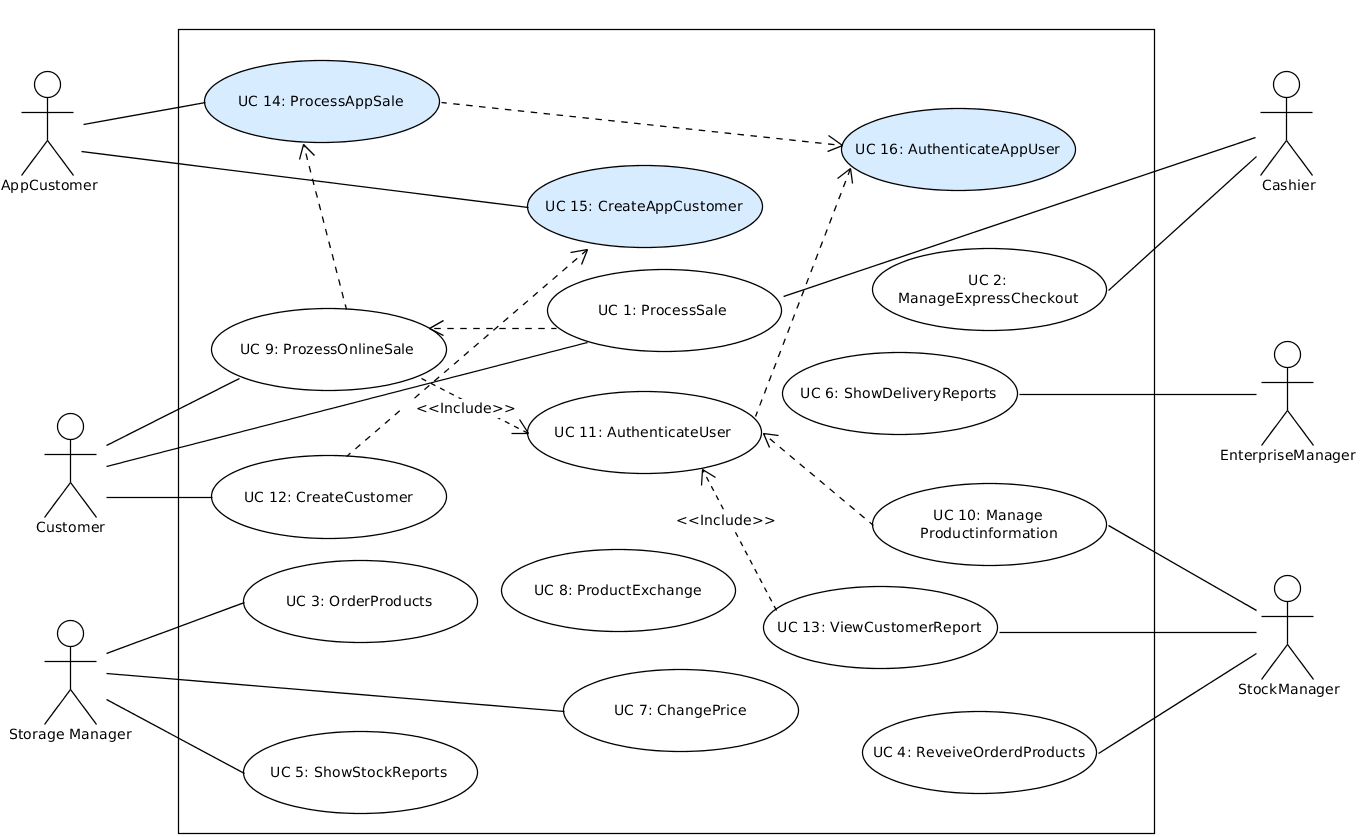
\includegraphics[width=\textwidth]{img/appUseCase.png}
			\caption{Use Case Diagram CoCoME Mobile App}
		\end{figure}

\textbf{UC 14 - ProcessAppSale}\\
\textit{Brief Description} A Customer selects the product items s/he wants to buy and the payment by credit card is performed.\\ \newline
\textit{Involved Actors} AppCustomer, Bank\\ \newline
\textit{Precondition} The App is ready to process a new sale and the Customer already has an account registered in the System.\\ \newline
\textit{Trigger} The Customer opens the app and wants to buy product items.\\ \newline
\textit{Postcondition} The Customer has paid and the sale is registered in the inventory.\\ \newline
\textit{Standard Process}
\begin{itemize}[leftmargin=*]
	\item[1.] The AppCustomer searches products provided by the App.
	\item[2.] The AppCustomer can see details for each product on a separate site.
	\item[3.] The AppCustomer adds the product items s/he wants to purchase to the Shopping Cart. Step 1-3 is repeated until all items are added to the cart.
	\item[4.] The AppCustomer gets an overview of the items in the cart, their price and the running total.
	\item[5.] The AppCustomer proceed to the Checkout 
	\item[6.] The AppCustomer selects the Store where s/he wants to pick up his/her	purchased product items. 
	\item[7.] The AppCustomer is presented with a login form and is required to complete the "Authenticate user" use case.
	\item[8.] In order to initiate card payment, the customer selects a credit card used for the purchase.
	\item[9.] The AppCustomer enters his/her PIN in the designated field presented by the System.
	\item[10.] The System presents the Customer with an overview of the purchase, the AppCustomer confirms the purchase and waits for validation. Step 9 is repeated until the validation is successful or the Customer decides to cancel the purchase.
	\item[11.] Completed sales are logged by the System and sale information are sent to	the Inventory in order to update the stock.
	\item[12.] A success message is presented to the AppCustomer and the product items
	are being prepared to be picked up by the customer.
	\item[13.] The AppCustomer closes the app.
\end{itemize}

\textit{Alternative or Exceptional Processes}
\begin{itemize}
	\item[-] In step 8: No Card available
	\begin{itemize}
		\item[1.] In order to add a new credit card the Customer clicks the Add Card button.
		\item[2.] The Customer enters the card number of the new credit card and saves the card.
	\end{itemize}
	
	\item[-] In step 10: Card validation fails
	\begin{itemize}
		\item[1.] The Customer tries again and again.
		\item[2.] Otherwise, the Customer can decide to cancel the purchase.
	\end{itemize}
\end{itemize}


\textbf{UC 15 - CreateAppCustomer}\\ \newline
\textit{Brief Description} The app offers a possibility to create a new Customer account.\\ \newline
\textit{Involved Actors} AppCustomer\\ \newline
\textit{Precondition} The Customer does not have a Customer account yet and the app is started.\\ \newline
\textit{Trigger} A new AppCustomer wants to create an account.\\ \newline
\textit{Postcondition} The User is authenticated.\\ \newline
\textit{Standard Process}
\begin{itemize}[leftmargin=*]
	\item[1.] The AppCustomer has to fill out forms, requesting all necessary information to create a new AppCustomer account.
	\begin{itemize}
		\item[(a)] Form for name, email and password
		\item[(b)] Form for address
		\item[(c)] Summery of the information 
	\end{itemize}
	\item[2.]The Customer fills out the forms, verifies and submits the information.
	\item[3.] The app verifies the given information and creates a new Customer account in the Inventory.
\end{itemize}

\textit{Alternative or Exceptional Processes}
\begin{itemize}
	\item[-] In step 3 : Provided information is incorrect or not valid. The Customer is notified of the problem and enters the information again until it passes the check.	
\end{itemize}

\textbf{UC 16 - AuthenticateAppUser}\\ \newline
\textit{Brief Description} The app provides the possibility to authenticate a User.\\ \newline
\textit{Involved Actors} AppCustomer\\ \newline
\textit{Precondition} The app is started.\\ \newline
\textit{Trigger} An AppCustomer wants to authenticate his/herself.\\ \newline
\textit{Postcondition} The AppCustomer is authenticated.\\ \newline
\textit{Standard Process}
\begin{itemize}[leftmargin=*]
	\item[1.] The AppCustomer gets displayed a login form. S/he is asked to enter email and password.
	\item[2.] The App checks the provided credentials. If correct, the AppCustomer is logged in.
\end{itemize}

\textit{Alternative or Exceptional Processes}
\begin{itemize}
	\item[-] In step 2: Wrong credentials
	\begin{itemize}
		\item[1.] An error message is displayed.
		\item[2.] The User may try again until the authentication succeeds.
	\end{itemize}
\end{itemize}


\newpage

\subsection{Design of the Mobile App}\label{DesignMobileApp}
 Fig. \ref{ComponentApp} is the component of this evolution scenario. When adding the Mobile App client, the hybrid cloud-based variant of CoCoME did not have to be modified. Therefore, CoCoME is encapsulated in a single component. Simply the three web services \textit{WebService::Inventory::LoginManager, WebService::Inventory::Store and WebService::Inventory::Enterprise} used by the App Client are emphasized. The entire component diagram for the hybrid cloud-based variant is available in the Technical Report \cite{HeinrichRostamiReussner2016_1000052688}. 
 \\ Fig. \ref{ComponentApp} indicates that the AppShop requires an adapter to access the web services provided by CoCoME. This is because CoCoME uses SOAP/WS*-based web services which are not compatible with the technology used to implement the AppShop Client. A more detailed introduction about the technology used to implement the Mobile App Client can be found in \cite{schnabel}. 
  
 \begin{figure}[!h]
	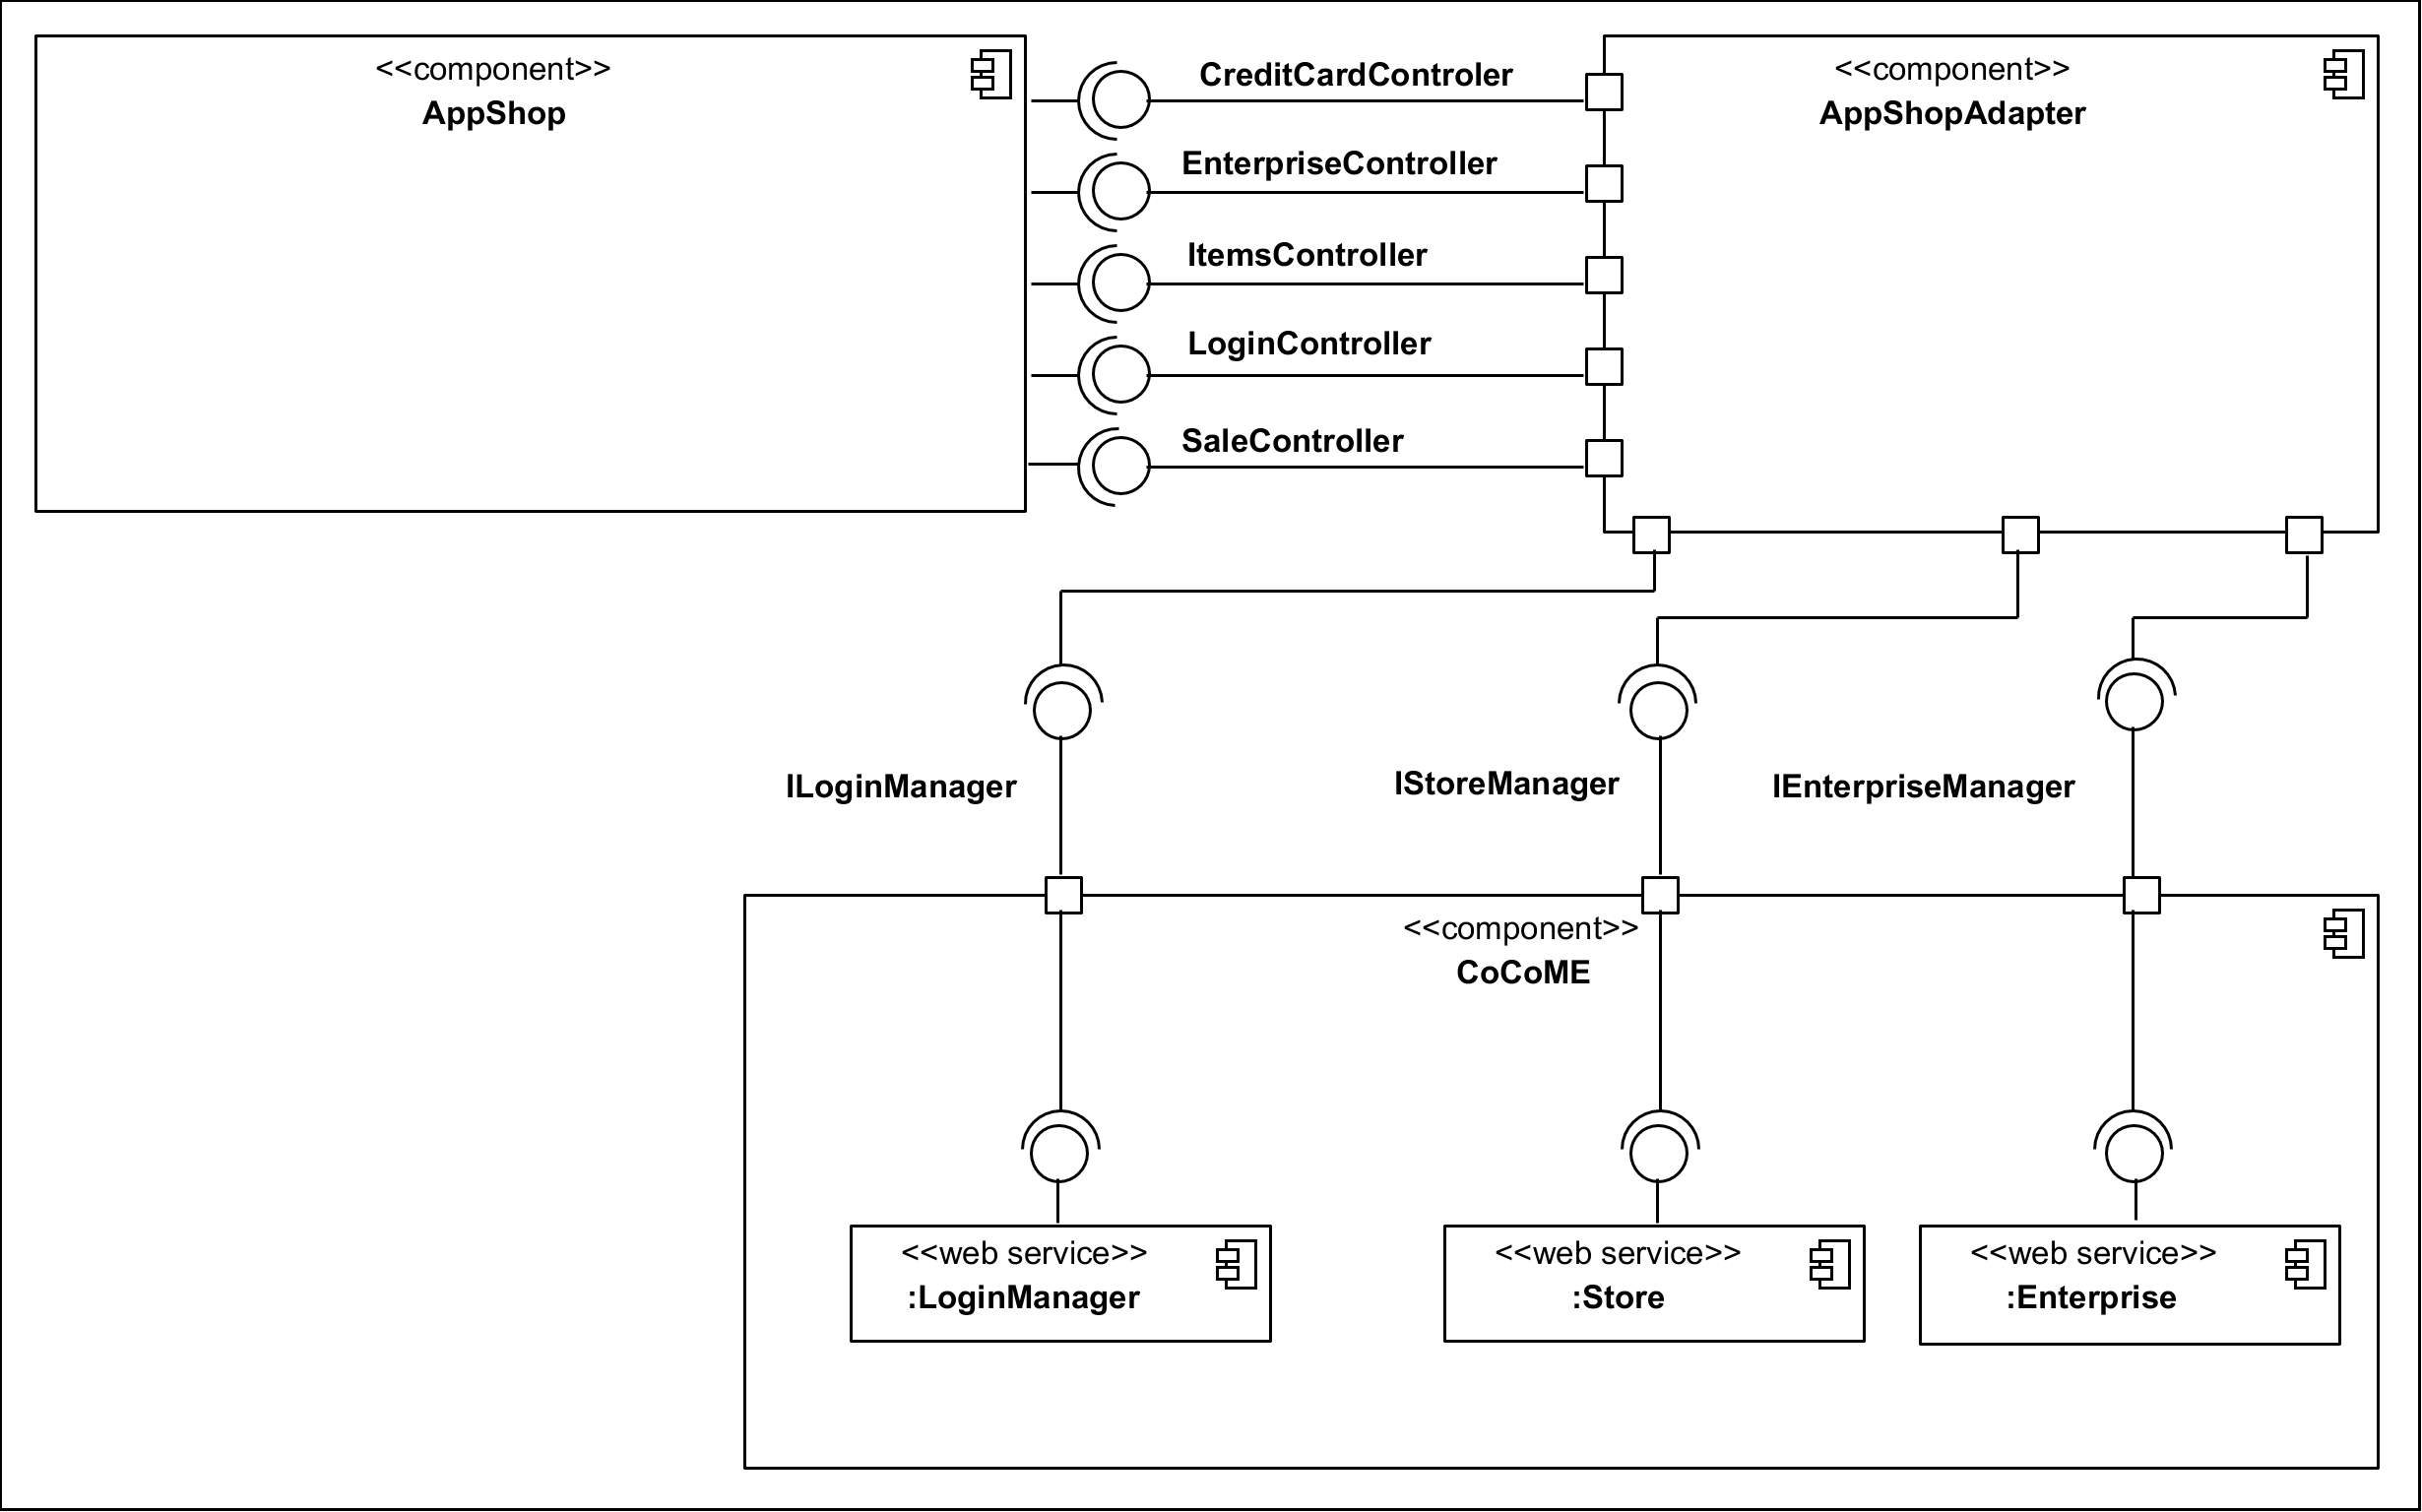
\includegraphics[width=\textwidth]{img/appComponent.png}
	\caption{Component Diagram of the CoCoME Ecosystem After Adding the Mobile App Client}
	\label{ComponentApp}
\end{figure}

  The \textit{AppShopAdapter} consumes the three web services \textit{WebService::Inventory::LoginManager, WebService::Inventory::Store} and \textit{WebService::Inventory::Enterprise} and provides a Rest Api which is used by the actual \textit{AppShop}. The Rest Api contains endpoints to retrieve and process Credit Card, Enterprise and StockItem information. To implement \emph{UC14-16}, the Api also provides endpoints for user management and processing sales. 
  
\begin{figure}[!h]
	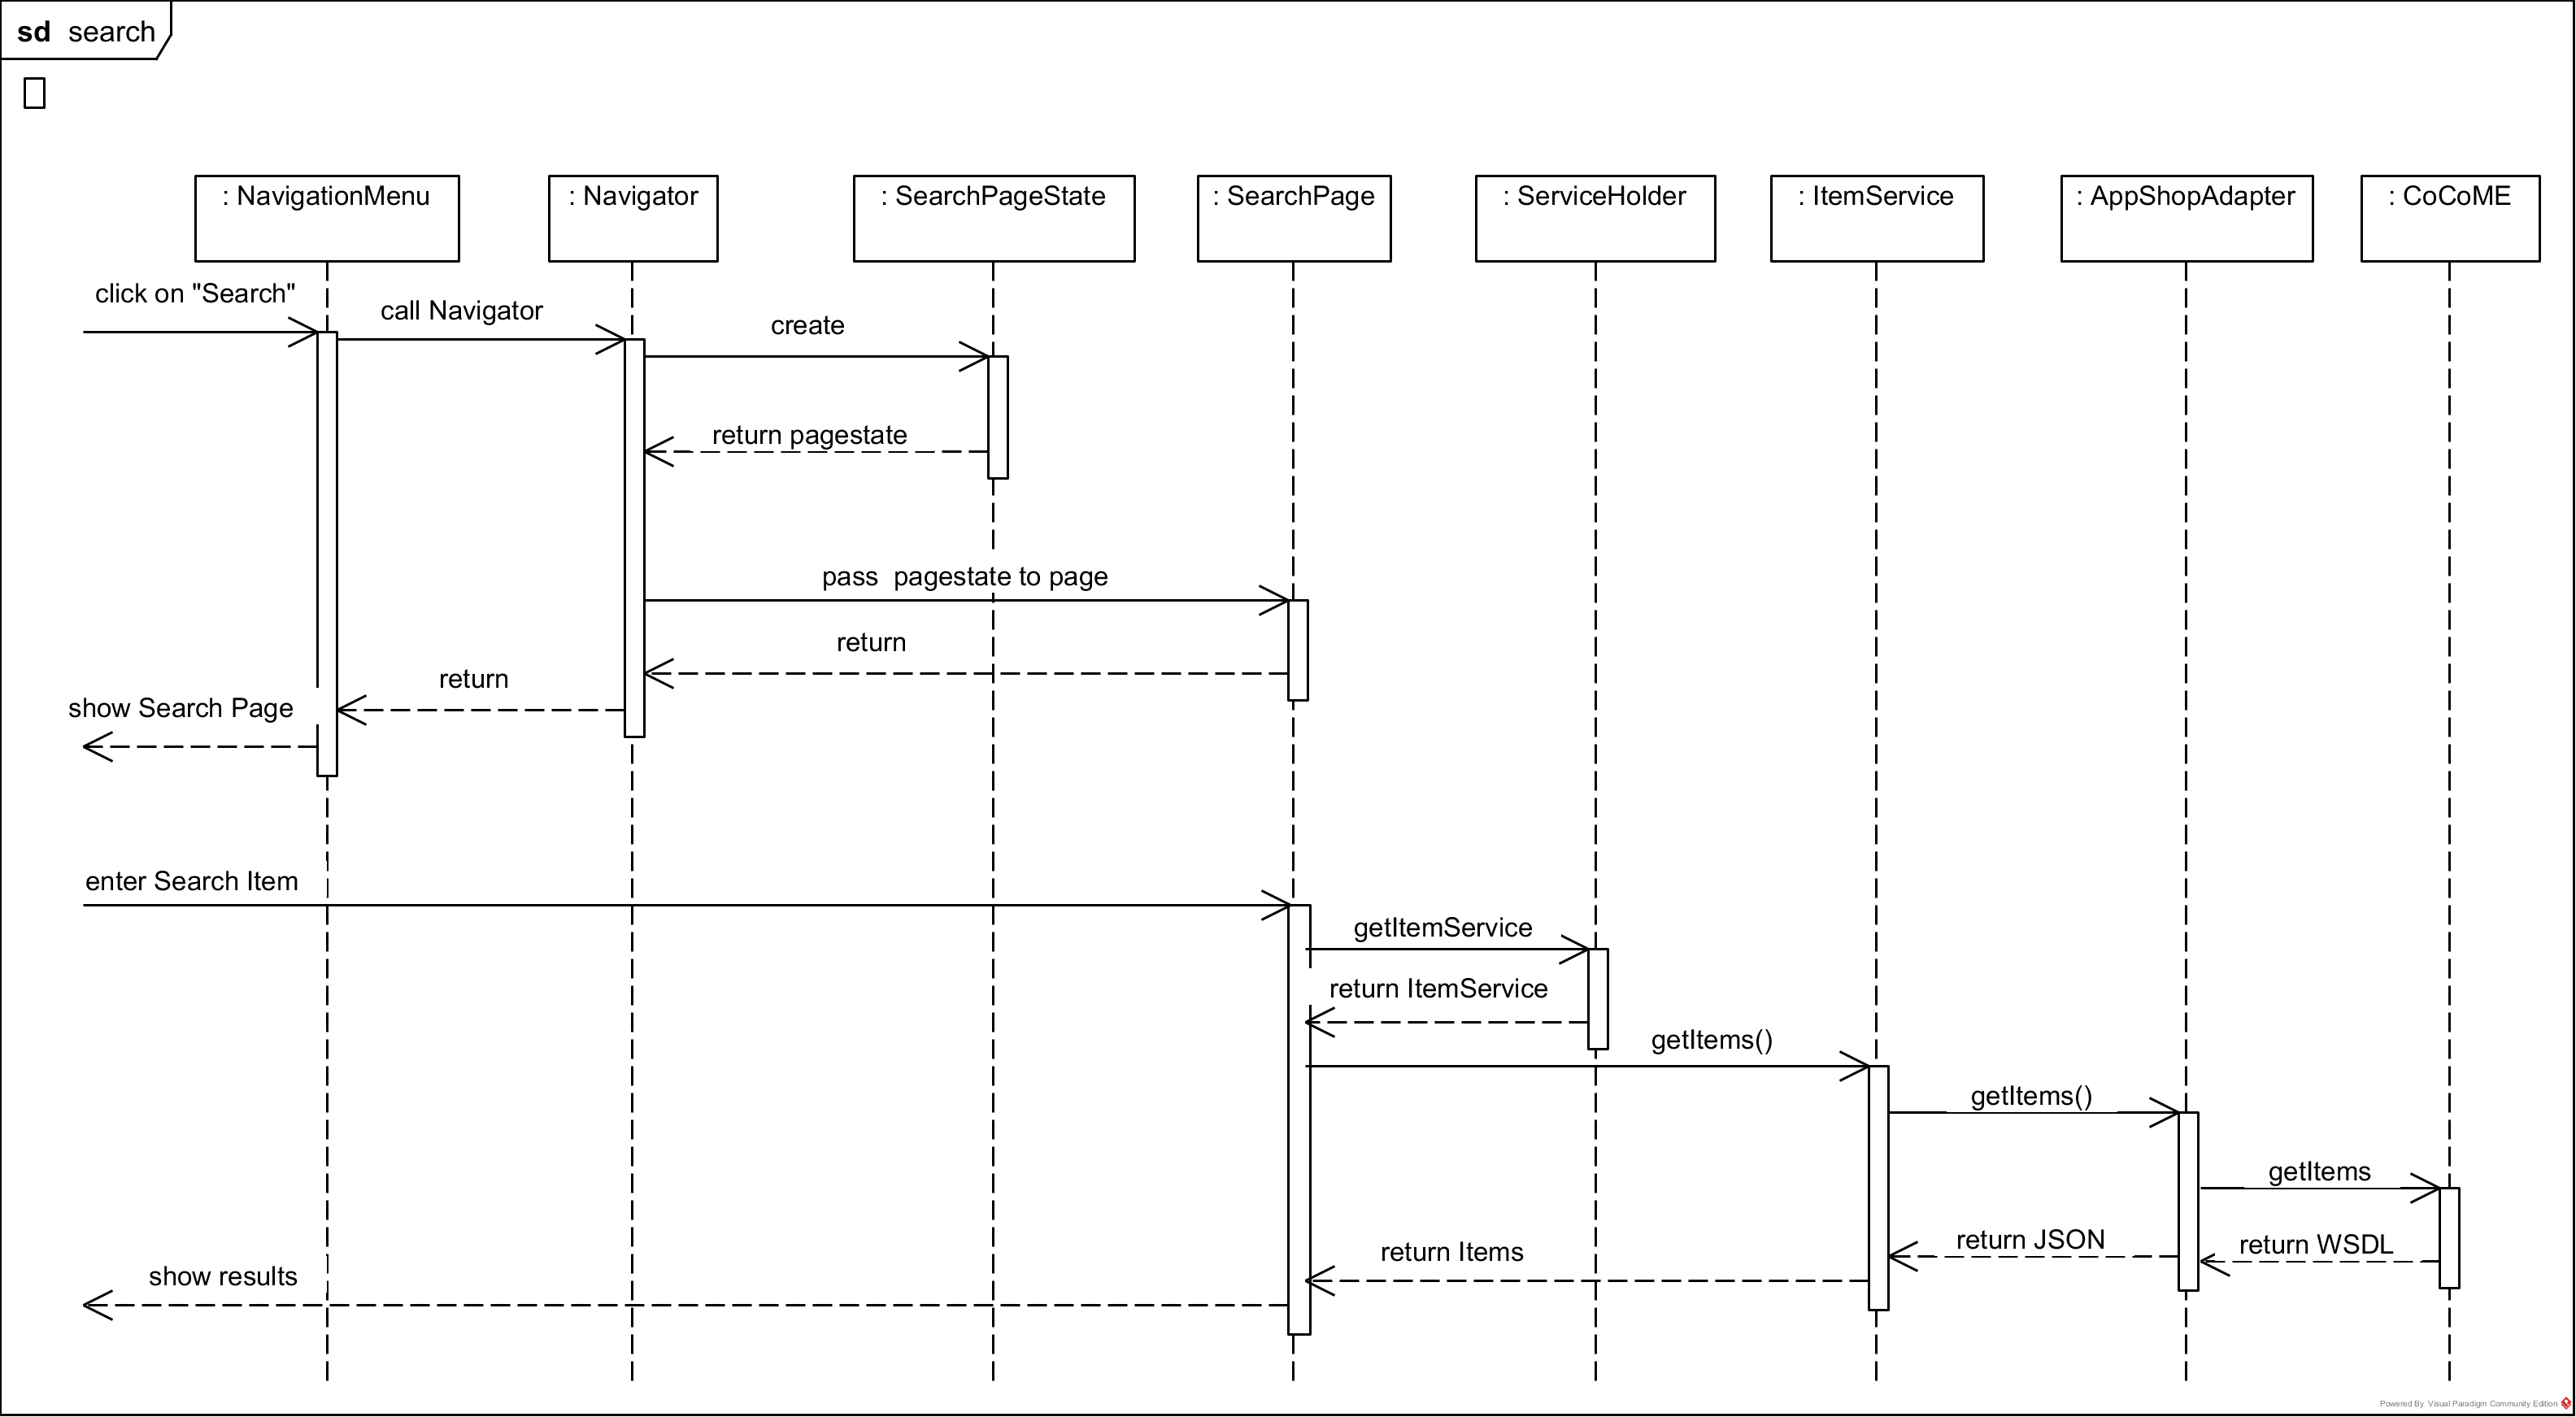
\includegraphics[width=\textwidth]{img/appSearchSequence.png}
	\caption{Sequence Diagram of Searching an Item in the Mobile App Client}
	\label{SequenceAppSearch}
\end{figure}

Fig. \ref{SequenceAppSearch} shows the process of opening a page to search for an Item. The customer opens the \textit{WebShopClient} and triggers the "Search" function to search for an item. To open the page, the \textit{NavigatorMenu} must call the \textit{Navigator} which creates a pagestate object and passes the object to the page. This HTML page is now presented to the customer. To fill the page with information, i.e when searching for a \textit{ProductItem}, the page uses services provided by the \textit{ServiceHolder}. In this case, the \textit{ItemService} calls the responsible REST-Service of \textit{AppShopAdapter} which in turn retrieves the necessary information from the WSDL services provided by CoCoME.


Fig. \ref{SequenceAppSale} demonstrates how the Mobile App Client processes sales.  For the sake of clarity, the digram is simplified and only contains the most important calls. First, the customer searches for items (according to Fig. \ref{SequenceAppSearch}). By clicking on the desired Item, the according \textit{ItemPage} is shown. This page carries information about the Item. Here, the customer decides whether the Item should be added to the Shopping Cart or not. The last steps are repeated until the customer decides to proceed to the checkout. If not logged in, the customer gets forwarded to the \textit{LoginPage}. When successfully logged in, the customer clicks the \textit{BuyNow}-Button. The Sale process is finished as soon as the backend (CoCoME) has processed the sale.




\begin{figure}[!h]
	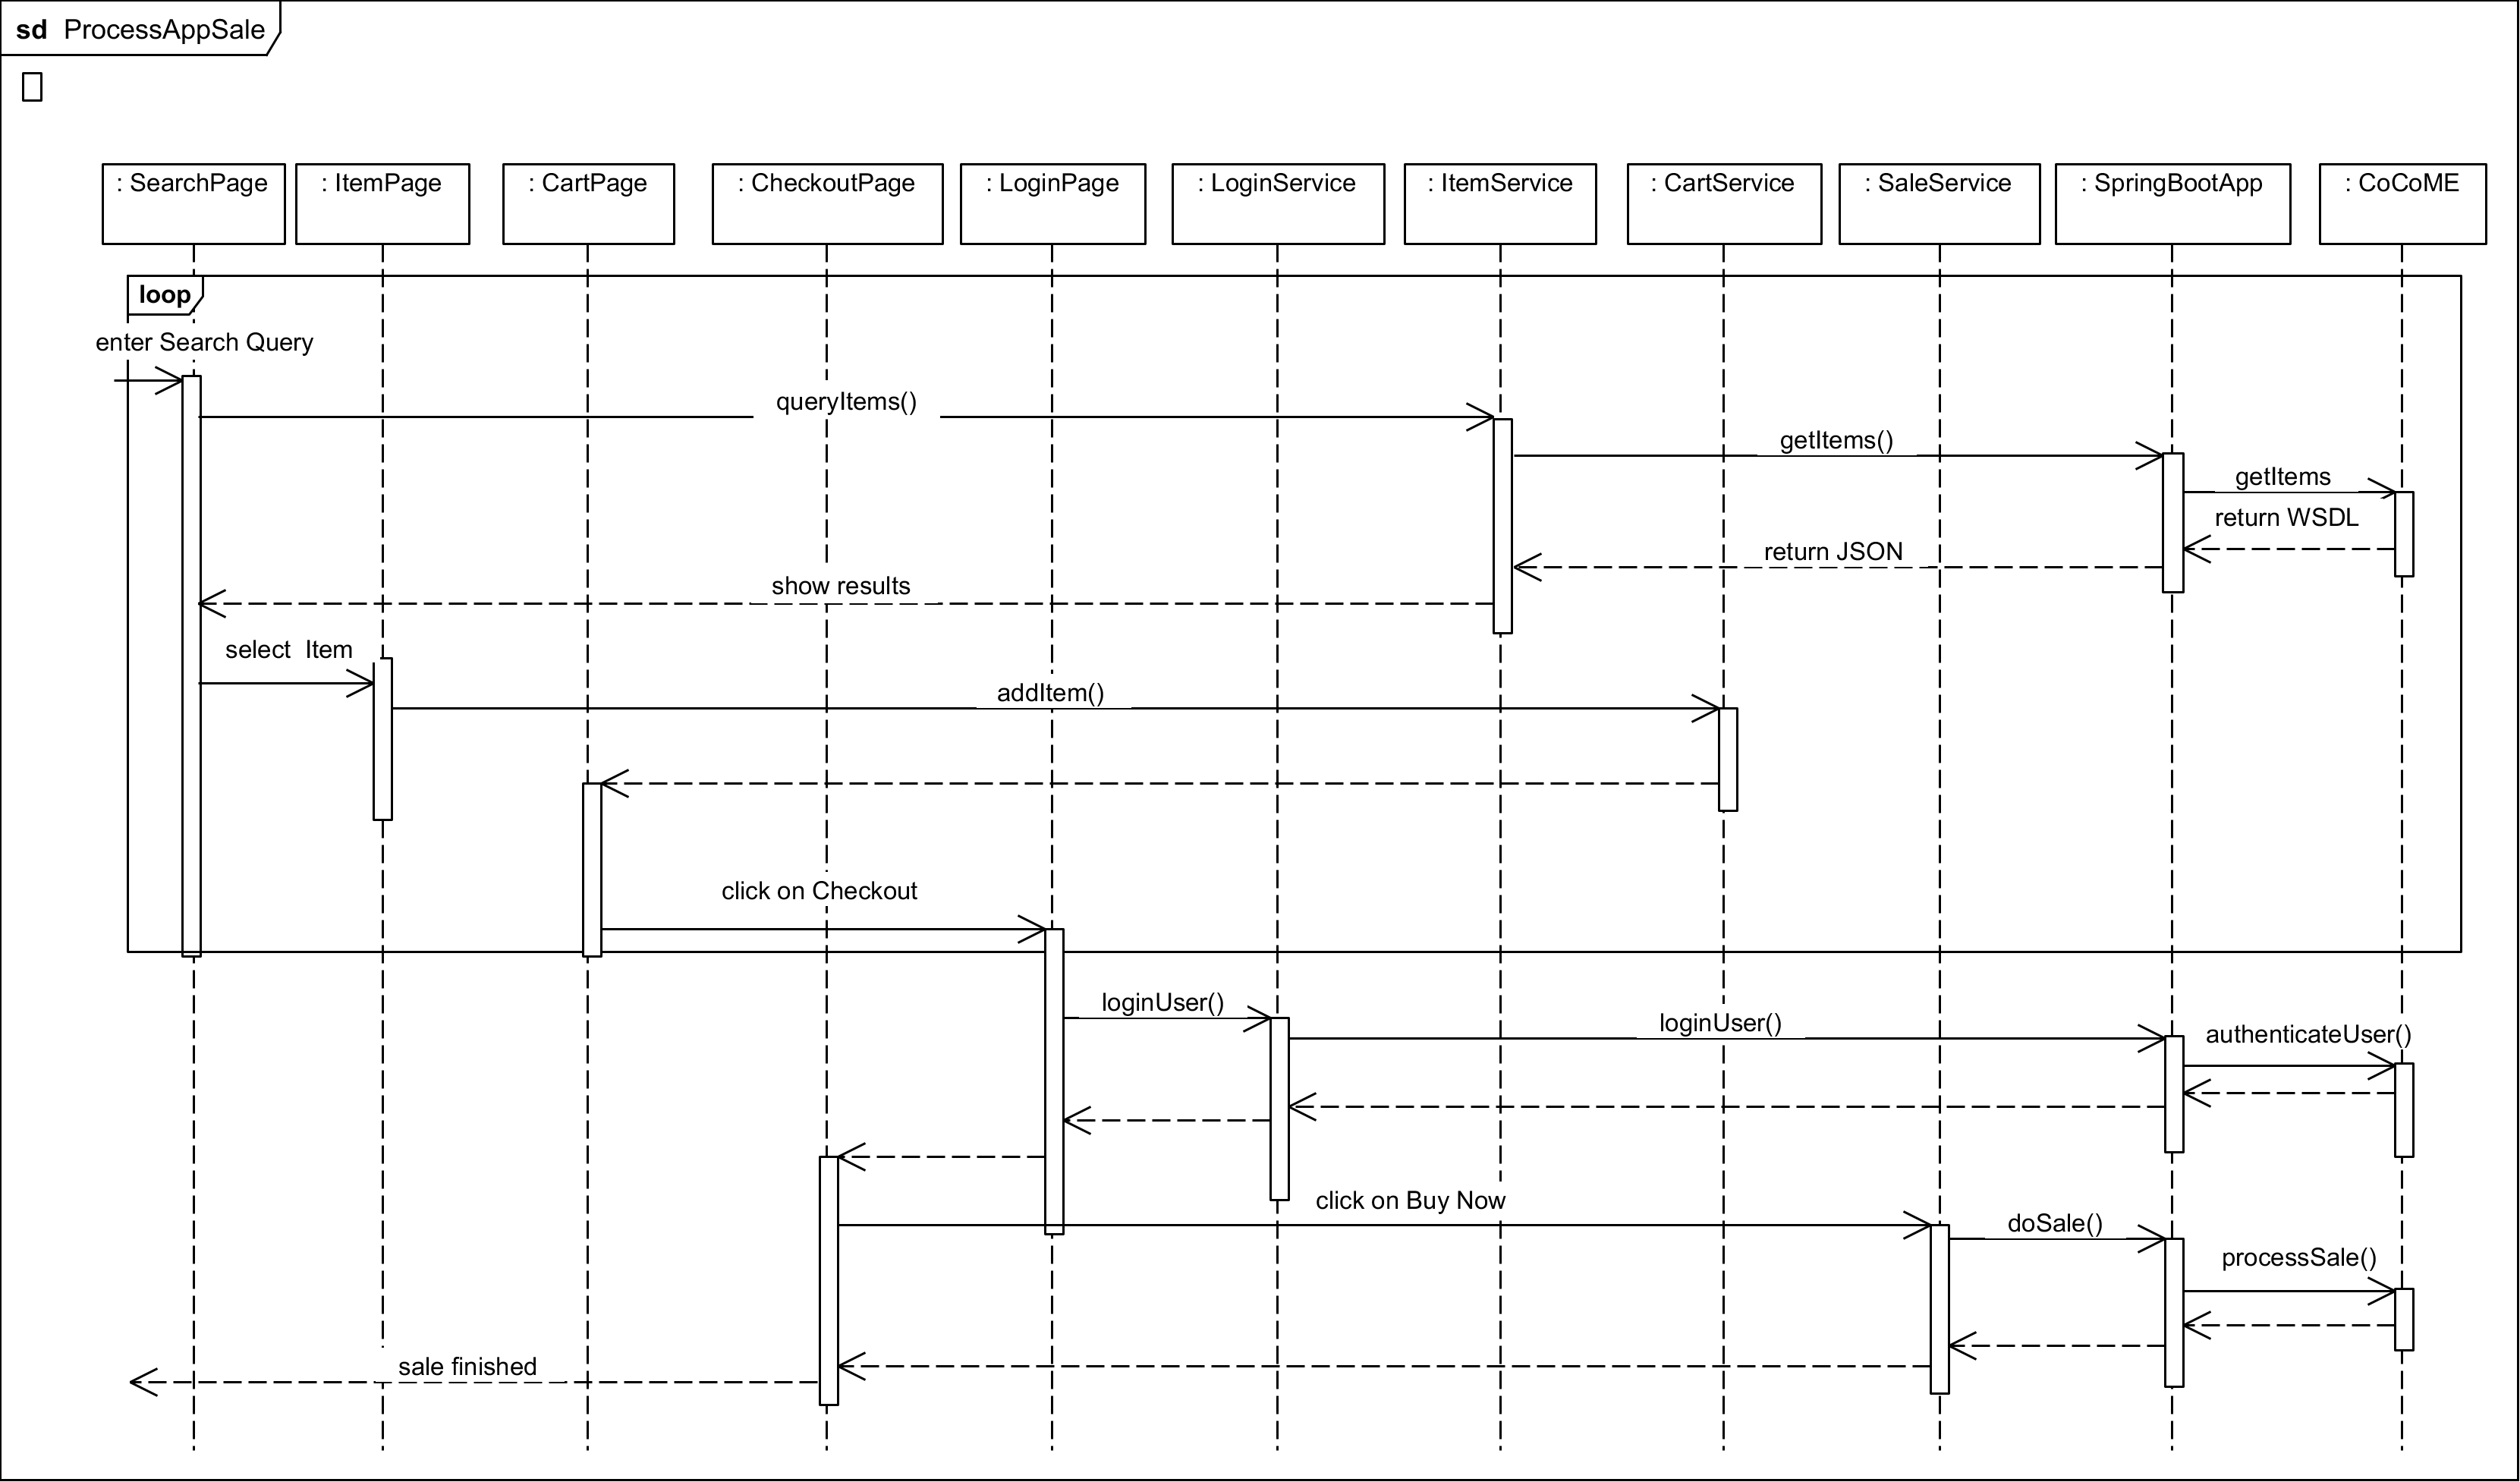
\includegraphics[width=\textwidth]{img/appProcessSale.png}
	\caption{Sequence Diagram of Processing a Sale}
	\label{SequenceAppSale}
\end{figure}

\newpage

\section{Using a Docker Environment} \label{Docker}

As shown in Fig. \ref{techStack}, using a Docker Environment affects the technology stack by adding additional layers. More detailed, the given CoCoME Stack is moved into the Docker Deamon, which runs a Linux distribution.The original parts of the stack, like Glassfish and the Java Virtual Machine, are still a part of the stack.
	
	\begin{figure}[!h]
		\centering
		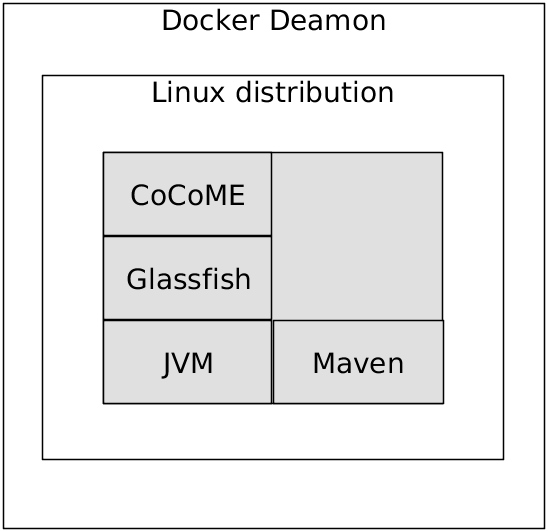
\includegraphics[width = 0.5\textwidth]{img/tech_stack_CoCoME.png}
		\caption{Extended technology stack CoCoME}
		\label{techStack}
	\end{figure}
	
The Dockerfile defines an environment based on the latest version of Ubuntu 16:04. Maven, Git and Java are also installed using the standard Ubuntu package manager.\\
Git has two purposes: On the one hand it is used to download the most recent version of CoCoME.	On the other hand, it is used to download a prefabricated version of Glassfish that already includes domains and other adjustments required for CoCoME. Java is required by Glassfish and CoCoME as they need the Java Virtual Machine. Maven is needed to deploy the latest version of CoCoME onto the provided Glassfish servers.
	
	
	During the development, it was decided to implement and provide two different versions. The first version always pulls the most recent CoCoME source code from GitHub, downloads the entire dependencies with Maven, compiles and builds the project and finally deploys CoCoME on the Glassfish servers. As a consequence, creating and starting a Docker Container takes about one hour.\\
	In contrast, the second version only pulls a prefabricated version of CoCoME from GitHub. 
	Therefore, pulling the source code up to building the project is skipped. Maven does not have to be included in the technology stack. Solely, deploying CoCoME on the Glassfish server is necessary.\\
	This reduces the deployment time to a few minutes but has a disadvantage: The prefabricated version is updated manually. Therefore, it is sometime not the most recent version.\\
	By providing both, a fast deploying version and a current version, the user can choose what's the best for its situation.
	

	

	
\section{Using Microservices Technology} \label{MS}

Info teils aus \cite{sommer}
	\begin{itemize}
		\item je microservice absatz mit entsprechenden Sequenzendiagram %fertig machen der implementierung
		\item frontend? muss dazu auch das gemacht werden?
		\item ein blocktext zu mehereren diagrammen oder diagramme zwischen text?
		
	
			\item je die einzelnen module und szenarien erlaeutern in dem diese sinnvoll sind
	\end{itemize}
	
		\subsection{Products}
		abstrahieren der Produktinformationen 
		
		\subsection{Stores}
		einzelne Laeden alleinstehend abbilden um nach bedarf neue microservices alias laeden starten zu können
		
		\subsection{Enterprise}
		aehnlich zu stroes
		
		\subsection{Reports}
		stellt alleinigen aufgaben bereich dar, entsprechen undabhaengig darzustellen von anderem.


	
	\chapter{Implementation of Evolution Scenarios}
This chapter describes implementation details for realizing the Docker environment \ref{DockerImplementation}, the Mobile App Client  for the existing hybrid cloud-based variant of CoCoME (\ref{AppImplementation}) and the Microservice-based variant (\ref{MicroserviceImplementation}).


\section{Using a Docker Environment}\label{DockerImplementation}
 	As shown in Fig. \ref*{Deploym_CoCoME}, the docker Container contains five different Glassfish servers. In particular they are called \textit{WEB}, \textit{ENTERPRISE}, \textit{STORE}, \textit{REGISTRY} and \textit{ADAPTER}. By default, Glassfish provides a Derby DB that is connected to the Service Adapter using Java Database Conectivity (JDBS) interface.
 	\begin{figure}[h]
 		\centering
 		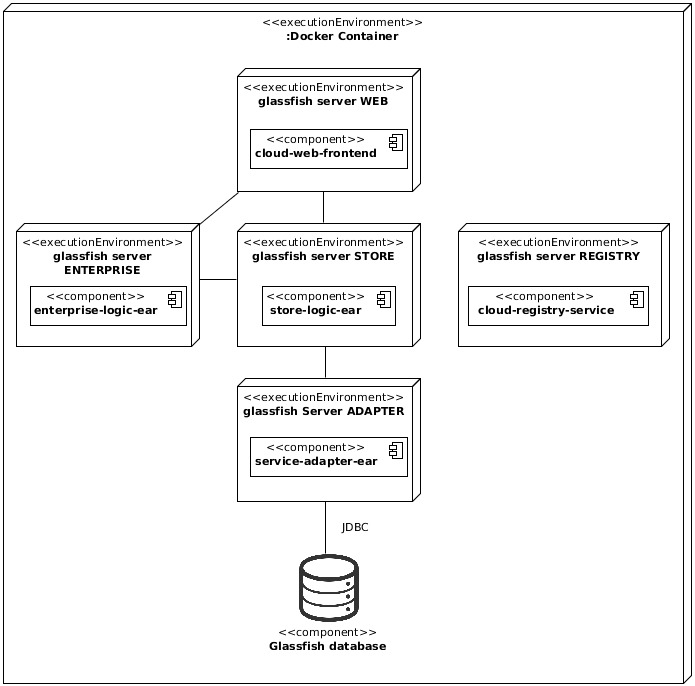
\includegraphics[width = 0.8\textwidth]{img/docker_Container_Deployment.png}
 		\caption{Deployment diagram CoCoME}
 		\label{Deploym_CoCoME}
 	\end{figure}
 	
 	The deployment assignment within the Docker environment is identical to the one specified in CoCoME deployment guide.
 	This means the maven generated archive files \textit{cloud-web-frontend},\textit{enterprise-logic-ear},\textit{store-logic-ear}\textit{cloud-registry-sevice} and \textit{service-adapter-ear} are deployed on the servers by using the following assignment:
 	\begin{figure}[H]
 		\centering
 		\begin{tabular}{p{0.25\textwidth}|p{0.01\textwidth}p{0.25\textwidth}}
 			Server && Deployment file \\
 			\hline
 			WEB && cloud-web-frontend  \\
 			ENTERPRISE && enterprise-logic-ear  \\
 			STORE && store-logic-ear  \\
 			REGISTRY && cloud-registry-service  \\
 			ADAPTER && service-adapter-ear \\	
 		\end{tabular}
 		\caption{Assignment of archive files to Servers}
 		\label{table_assignment}
 	\end{figure}
    As mentioned earlier, there are two versions of this Docker project.\\
 	 The fast version can be extended by the Pick-Up shop\footnote{\url{https://github.com/cocome-community-case-study/cocome-cloud-jee-web-shop}}. This Pick-Up shop runs inside a separate Docker container which is shown in figure \ref{Deploym_Pickup}.  
 	\begin{figure}[h]
 		\centering
 		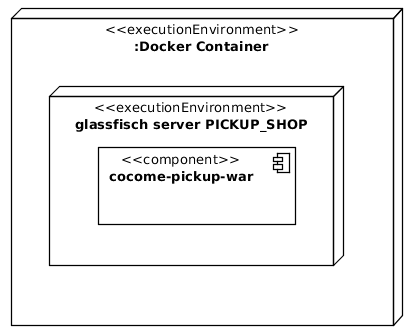
\includegraphics[width = 0.4\textwidth]{img/docker_Container_PickUP.png}
 		\caption{Deployment diagram CoCoME Pickup Shop}
 		\label{Deploym_Pickup}
 	\end{figure}
 	As shown in figure \ref*{Deploym_Pickup}, this container provides only one Glassfish server.
 	\begin{figure}[H]
 		\centering
 		\begin{tabular}{p{0.25\textwidth}|p{0.01\textwidth}p{0.25\textwidth}}
 			Server && Deployment file \\
 			\hline
 			PICKUP\_SHOP && cocome-pickup-war \\	
 		\end{tabular}
 		\caption{Assignment archive files to Servers}
 		\label{table_assignment_pickup}
 	\end{figure}
 	To control the start of both containers, precisely the CoCoME and the Pick-Up Shop, another specific file is needed: the Docker Compose file. It ensures that the CoCoME Container is active, before the Pick-Up Shop container starts. This is necessary as the Pickup Shop requires a running instance of CoCoME to register itself.\\
 	Whereas CoCOME does not require the Pick-Up Shop, the inversion is not corrext.
 	Both containers need to communicate with each other. By default, docker prohibits any outgoing and ingoing communication from and in a container. This is solved by opening specific ports through which the communication is possible. Which ports the containers can use is specified in the Docker Compose file as well.
 	
 	
 \section{Adding a Mobile App Client}\label{AppImplementation}
 Adding a Mobile App Client did not require a modification within the hybrid cloud-based variant of CoCoME. The implementation was done using the Cordova framework and OnsenUI to provide a multi OS compatible backend and UI \cite{schnabel}. The App itself is written in Typescript/Javascript. Fig. \ref{App_ClassDiagram} shows the principal classes and their relationships.
 \\
  The \textit{Navigator} is the primary class that manages the pages. The pages consist of two components: The \textit{Page} itself and its \textit{PageState}. The \textit{PageState} is used to store and transfer the current status of a page. There are currently six different pages available: \textit{IndexPage}, \textit{SearchPage}, \textit{ItemPage}, \textit{CheckoutPage}, \textit{CartPage} and \textit{LoginPage}. For the sake of clarity, they are subsumed under the generic terms \textit{ConcretePage} and \textit{ConcretePageState}. 
  \\
  Pages use components. Such components are i.e. the \textit{Navbar} or the \textit{Searchbar}. These components are abstract descriptions of UI elements that are connected to the actual \textit{HTML-elements} via Knockout.js. By using Knockout.js, changing values of a component results in an immediate change of the UI. 
  Besides, the App Client retrieves information of the CoCoME system.  As mentioned in \ref{DesignMobileApp}, the Client is not able to access the CoCoME system directly. Therefore, the pages use \textit{Services} provided by a \textit{ServiceHolder} to call the \textit{AppController'} Rest-API. The \textit{AppController} is written in Java using the SpringBoot framework and converts the Rest-requests of the App Client to SOAP-Requests in order to match the CoCoME-API. 
  
  
   \begin{sidewaysfigure}[ht]
  	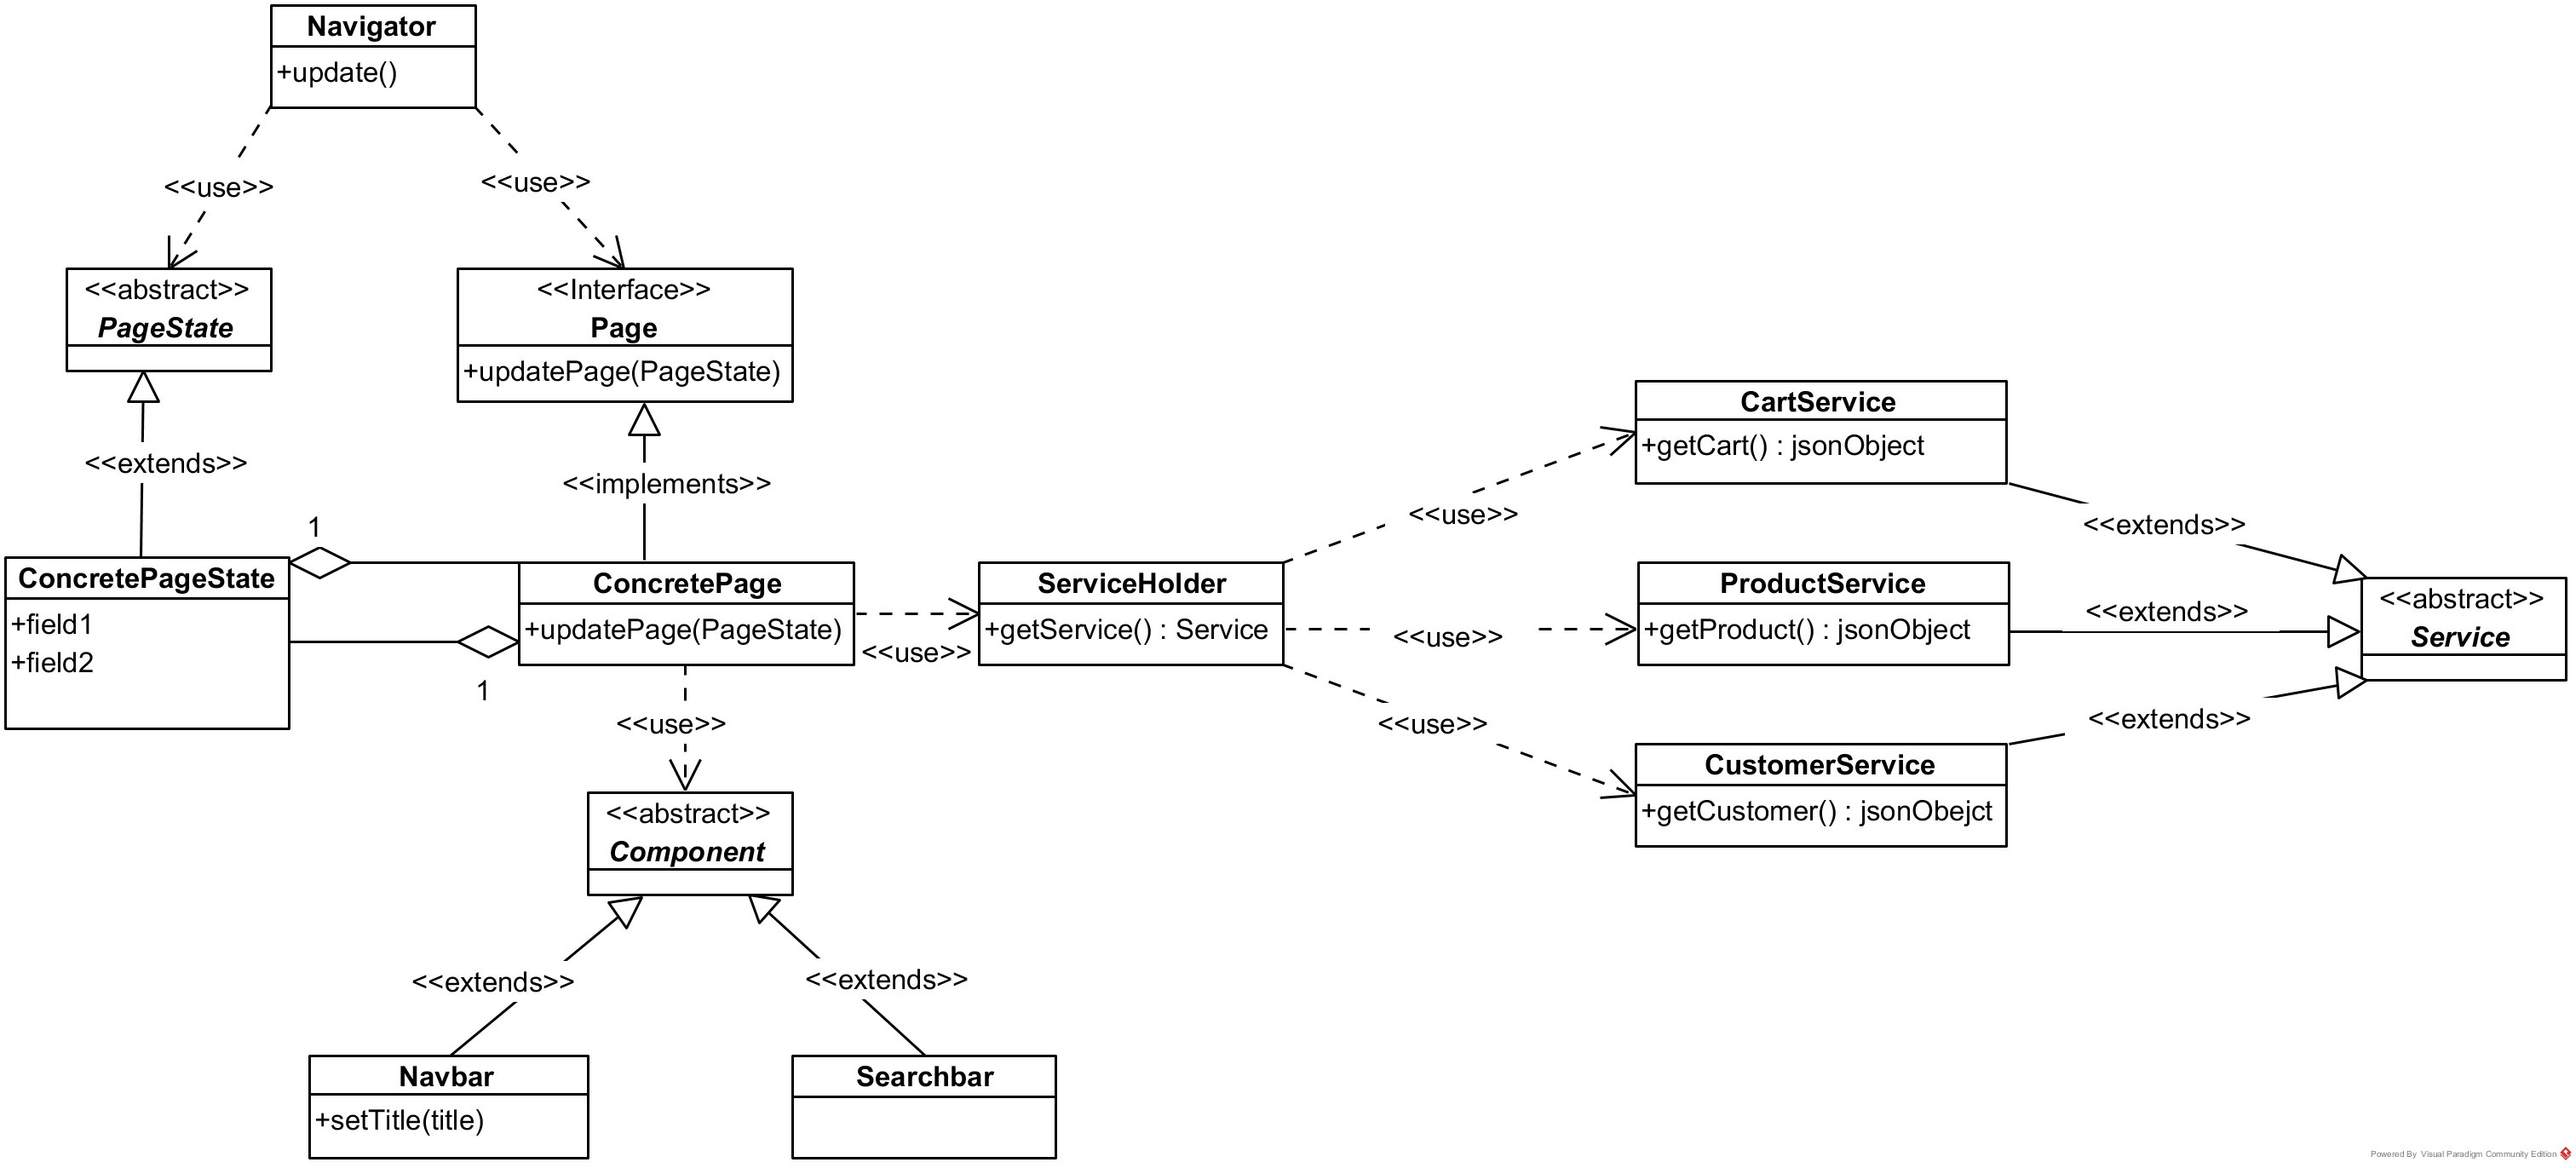
\includegraphics[width=\textwidth]{img/appBasicClass.png}
  	\caption{Primary Classes of the App}
  	\label{App_ClassDiagram}
  \end{sidewaysfigure}

\FloatBarrier
 
 
 \section{Using Microservice Technology}\label{MicroserviceImplementation}
 
\begin{figure}[h]
	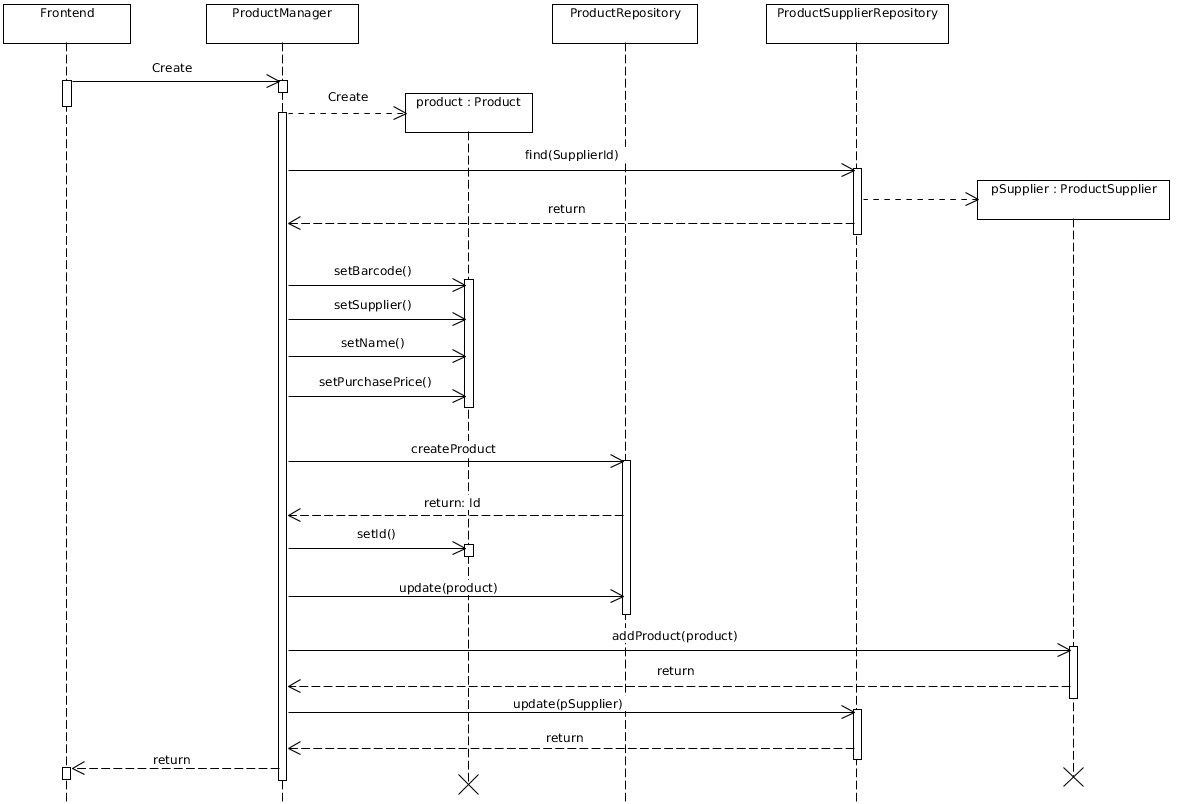
\includegraphics[width = \textwidth]{img/seqProductCreate.png}
	\caption{Sequence Diagram \textit{Creating a new Product}}
	\label{seqCreateProduct}
\end{figure}

\begin{figure}[h]
	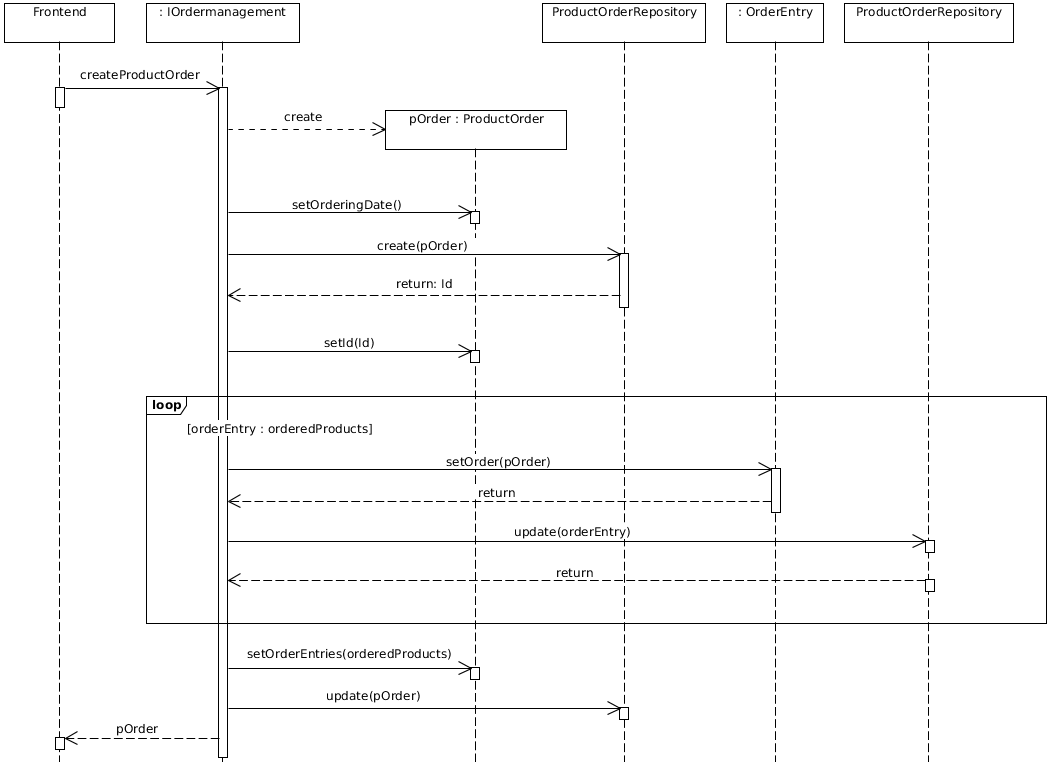
\includegraphics[width = \textwidth]{img/SeqProductOrderEntry.png}
	\caption{Sequence Diagram \textit{Creating new Product Order}}
	\label{seqProductOrder}
\end{figure}
	
	
	
	%
	% ---- Bibliography ----
	%
	\nocite{*}
	\bibliographystyle{abbrv}
	\bibliography{literatur}
	
	\sloppy
\end{document}